%!TEX root = index.tex
\chapter[Metodologia]{Metodologia}
\label{chap:metodologia}

\begin{figure}[h]
\caption{Metodologia Utilizada no Trabalho}
\centerline{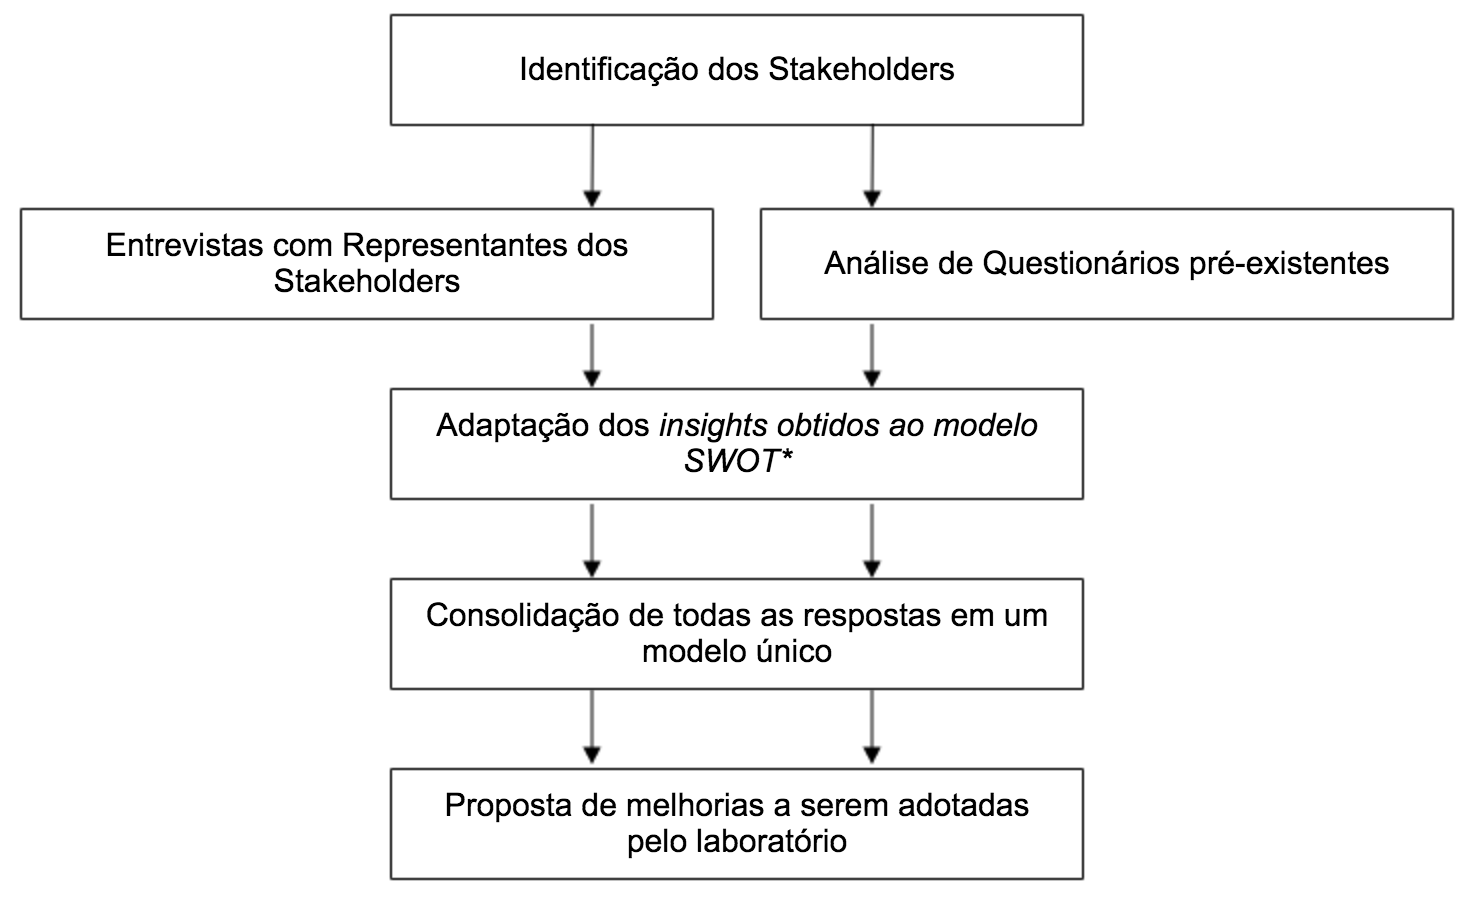
\includegraphics[scale=0.5]{img/metodologia}}
\label{fig:metodologia}
\caption* {Fonte: Elaborado pelo próprio autor}
\end{figure}

Após conversas iniciais com membros da Samsung e do PRO, foram definidos os stakeholders do projeto Ocean. Foram identificadas pessoas-chave em cada um dos \textit{stakeholders} para serem feitas entrevistas pessoais gravadas, sem questionários previamente fechados para deixar o entrevistado livre para comentar além do que foi perguntado. Coube ao entrevistador guiar a conversa para manter a conversa sempre próxima ao escopo do laboratório.

Para um \textit{stakeholder} específico, que são os frequentadores dos cursos oferecidos pela Samsung, foram utilizados modelos analíticos para extrair informações de questionários previamente respondidos ao longo da execução dos cursos nos anos de funcionamento do Ocean. Insights obtidos a partir desses modelos analíticos também são de grande valia para a Samsung, pois esse material nunca havia sido explorado anteriormente. Para usuários de cursos intensivos, foram feitas entrevistas com representantes de \textit{startups} que frequentaram o curso anteriormente, centradas na pergunta: "Como a participação no curso intensivo mudou a vida da empresa e as vidas dos participantes?".

Foi utilizada uma adaptação do modelo SWOT para ilustrar as percepções obtidas de cada stakeholder, a qual difere do modelo original do SWOT por não se tratar de uma análise de negócio baseada em fatores de mercado e competitividade, e sim em uma análise fria e absoluta de oportunidades de melhoria e identificação de problemas. Foi considerado que por ser um modelo simples e de fácil visualização, consolidaria as necessidades deste trabalho sem desvirtuar os objetivos propostos.

A partir dos resultados obtidos pela análise das respostas, trabalhou-se em cima da geração de propostas de melhoria.